\chapter{Fundamentação teórica e metodologia}

\section{\dBG}

% - Detailed explanation of \dBG of a set of DNA sequences
%   - reverse complements
% - How it is going to be used
% - Operations
%   - Insert node
%   - Insert edge
%   - Query node
%   - Query edge / star 
% - Space-efficient representations - that's what we propose

The \dBG is a directed graph for which each node represents a sequence of symbols, and each edge between two nodes represents
the overlap between the two sequences. That is, given two nodes on the graph, they each represent a distinct sequence of symbols
$S_1$ and $S_2$, and there is an edge between them if and only if the tail of $S_1$ is the head of $S_2$.

Within the context of genome sequencing, \dB graphs are used in the assembly process by storing the distinct \kmers identified
in the read sequences. In the ideal case (when each \kmer is present only once in the original sequence, and there are no
sequencing errors), the complete traversal of this graph would produce the original sequence. In practice, such a straightforward
approach is not feasible, but the \dBG can still be used to produce longer sequences, called \emph{contigs}, which can then be processed
to assemble the original genome. Figure~\ref{fig:dbgexample} presents an example of the \dBG within this context.

\begin{figure}[htbp]
	\begin{center}
    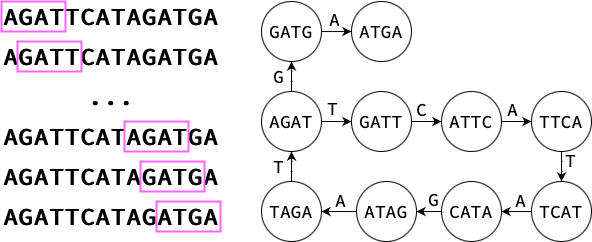
\includegraphics[width=0.8\textwidth]{figures/dbg-example}
	\end{center}
	\caption{Example of a \dBG. $k=4$}\label{fig:dbgexample}
\end{figure}


\subsection{Representing a \dBG}

\asq{Não é mais interessante manter a discussão sobre lower boundaries no capítulo de estado da arte?}

Due to its nature, a \dBG can be represented by its set of nodes or edges independently, as one can be derived from the other.
\asq{Citation needed?} As such, a structure that can answer queries about the presence of a given node on the graph is enough to
represent the graph\footnote{Conversely, the same can be achieved with a structure that can answer the same kind of query but about
edges. Such structures are called edge-centric, as opposed to the node-centric structures that we consider in this work. Both versions
are trivially equivalent, however.}. In this regard, Conway \& Bromage showed that a lower bound on the number of bits required to
\emph{exactly} represent a \dBG exists, and is $\Omega(n \log n)$, for $n$ being the number of distinct \kmers present in the graph,
and $4^k > n$\cite{Conway2011}.

In order to further improve space-efficiency, new forms of representation were created that trade exactness for a probabilistic approach,
such as \emph{Navigational Data Structures} (NDS), which have some probability of giving an erroneous answer to a membership query, 
but can be used to navigate the graph. This definition is useful due to the fact that a \dBG is not queried for the membership of randomly
selected nodes, but rather only the neighborhood of a known member node is queried\cite{Chikhi2014}. In the same paper where they introduce
the idea of NDS, Chikhi \emph{et al.} also present a lower bound for the number of bits needed to represent such a structure as $3.24n$.
In sections \ref{sec:debruijncountmin} and \ref{sec:debruijnhashtable} we will introduce two new NDS's. \asq{É necessário reiterar
os objetivos das duas estrutas aqui, visto que isso já seria feito na introdução e é feito nas próprias sessões dedicadas a cada estrutura?}

\subsection{Reverse Complements}

One individuality of the genome sequencing context is the presence of \emph{reverse complements}. When generating sequencing reads,
a sequence of DNA can be read both in its forward form, or in its reverse complement. That is, the read is generated not from the
original sequence $S$, but its complement $\overline{S}$, generated by swapping each base with its Watson-Crick complement
($\A \leftrightarrow \T$, $\C \leftrightarrow \G$). As in \cite{Conway2011}, this will be treated by processing all reads in both
directions, without, however, merging nodes representing reverse complements. As noted by Conway \& Bromage: ``This makes the graph
symmetric; a forward traversal corresponds to a backwards traversal on the reverse complement path, and vice versa.``\cite{Conway2011}.


\section{\cm}
\label{sec:countmin}

The \cm sketch, first introduced in \cite{Cormode2005}, is a sub-linear data structure intended to allow for event frequency mapping.
In this way, it must allow for the query of the frequency of a given event, as well as the update of that frequency, through the
\emph{query} and \emph{update} operations. The sketch is composed of a $W$-wide, $D$-deep matrix of counters. With each row in this
matrix is associated a hash function that map the possible events to the $W$ positions in that row. All $D$ hash functions
must be pair-wise independent.

Updating the frequency of a given event is done by passing it through the hash functions for each row, and then updating the counter in
the resulting position accordingly. \toconsider{In this work we take interest in a simpler version of the \cm sketch where the counters
are only incremented by one.}

Querying the structure consists of, similarly, retrieving the value of the counter associated with the key in each row, and then returning
the minimum value among them.

Figure \ref{fig:countminexample} presents a visualization of the \cm sketch.


\begin{figure}[htbp]
	\begin{center}
    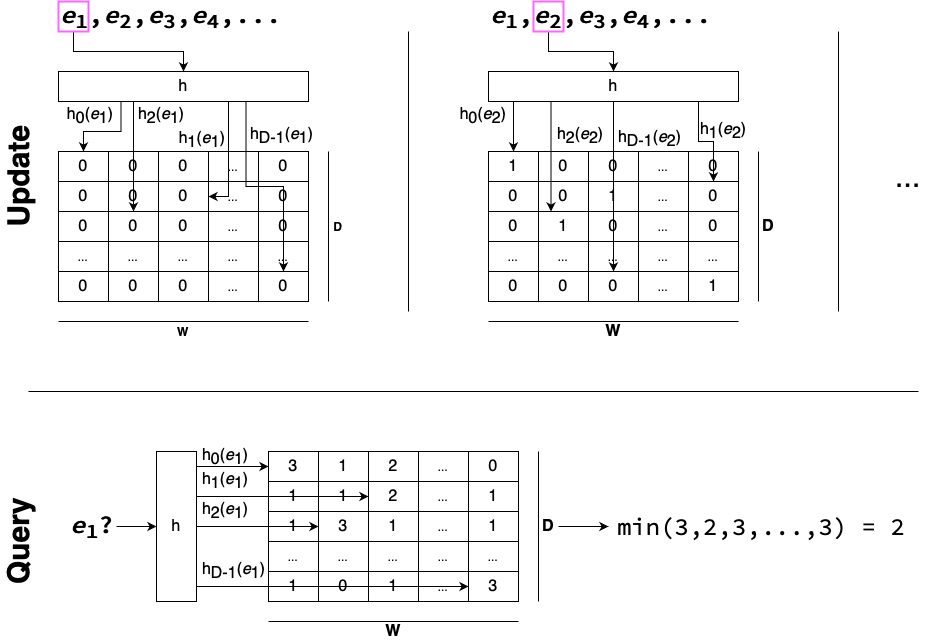
\includegraphics[width=0.8\textwidth]{figures/cm-example}
	\end{center}
	\caption{Example of a \cm sketch being used to count \kmers. $k=4$}\label{fig:countminexample}
\end{figure}

\subsection{As a representation for a \dBG}

\asq{Vale colocar isso aqui, ou é mais interessante deixar apenas para falar disso no capítulo anterior (State of the Art), quando falando
sobre o \emph{FastEtch}?}

A \cm sketch can implement the membership query operation by querying the count for a given \kmer and comparing it to a presence threshold:
if the count surpasses this threshold, the \kmer is considered to be present in the \dBG, and if the count is inferior to the threshold the
\kmer is considerent absent from the graph. The MEMB function is defined in Algorithm \ref{alg:countmin-memb}.

\begin{algorithm}[htbp]
  \caption{MEMB}\label{alg:countmin-memb}
  \KwData{$\kmer$; $\mathit{sketch}$, the \cm sketch, $\mathit{threshold}$, the threshold for the presence of a \kmer in the \dBG}
  \Return{$\mathit{sketch}.query(\kmer) \geq \mathit{threshold}$}
\end{algorithm}

\section{\dBCM}
\label{sec:debruijncountmin}

% - Representation (what goes in each cell)
% - Operations:
%   - addOutEdge
%   - query 
% - Analysis space/time (may be done within previous sections)

\asq{Como nós vamos falar das out-edges tanto no \dBCM quanto no \dBHT, poderia ser interessante fazer uma sessão ou subsessão acima
falando sobre o conceito de forma que ele seja apenas referenciado nessas sessões?}

In order to leverage the benefits of using a \cm representation of the \dBG while also improving its navigability, we introduce a modified
version of the \cm sketch, which we call the \dBCM, that allows the sketch to be queried not only for \kmer counts, but also for the
out-edges from the \dBG associated with that \kmer. \toconsider{The goal with this modification is to reduce the number of false positives
by querying only the neighbors that are known to possibly exist for that \kmer. This would avoid false paths to be traversed, improving
the trustworthyness of the graph.}

To store the additional information, we expand the \cm sketch such that each cell in the matrix stores not only the counter,
but also a set of out edges. The structure, then, provides an interface to increment the counters associated with a given key by one,
and an interface to add an out edge to the sets associated with a given key. The increment operation is performed in the same way as in
a regular \cm sketch, and the algorithm for the add edge operation can be seen in Algorithm \ref{alg:addOutEdge}.

Furthermore, the \dBCM must accomodate this new information in its query operation. In order to do this, the sketch returns not only
the minimum value of the counters, but also the intersection of the sets of out edges. The algorithm for the updated query operation is
described in Algorithm \ref{alg:query}.

\begin{algorithm}[htbp]
    \caption{Add an out-edge to a \kmer in a \dBCM}\label{alg:addOutEdge}
    \KwData{$\mathit{outEdge} \in \{\A, \C, \G, \T\}$}
    \For{$i = 1, \ldots, D$}{
      $\mathit{CountMin}[i][h_i(\text{k-mer})].\mathit{outEdges} \gets \mathit{CountMin}[i][h_i(\text{k-mer})].\mathit{outEdges} \cup \mathit{outEdge}$\;
    }
\end{algorithm}

From a practical perspectie, due to a node only ever having 4 possible out edges (corresponding to the 4 bases $\{\A, \C, \G, \T\}$),
the set of out edges can be represented by a bit vector indicating whether each of these possible edges is present. An edge is added
by setting the corresponding bit, and the intersection is obtained by performing the bitwise AND operation. This allows both set of
out edges and the counter to be stored together in a single integer. \toconsider{When using a $k$ such that $4^k > |S|$, the each \kmer in $S$
is expected to appear only once. As such, it is expected to appear $C$ times in the reads. Considering that $C$ is not a very high value
(commonly below $200$} \asq{Citation Needed?}\toconsider{), each counter can be represented by a 12-bit integer, accounting for the expected count for
all real \kmers, as well as any possible collisions.}

\begin{algorithm}
    \caption{Query a \kmer in a \dBCM}\label{alg:query}
    $\mathit{count} \gets \mathit{inf}$\;
    $\mathit{outEdges} \gets \{\A, \C, \G, \T\}$\;
    \For{$i = 1, \ldots, D$}{
      $\mathit{count} \gets \min(\mathit{count}, \mathit{CountMin}[i][h_i(\text{k-mer})].\mathit{count})$\;
      $\mathit{outEdges} \gets \mathit{outEdges} \cap \mathit{CountMin}[i][h_i(\text{k-mer})].\mathit{outEdges}$\;
    }
    \Return{$(\mathit{count}, \mathit{outEdges})$}
\end{algorithm}

\subsection{As a representation of a \dBG}

As with the \cm sketch, a \dBCM sketch can be queried for membership by comparing the count associated with a given \kmer to a threshold
for presence (i.e. the \kmer is considered present if it appeared more than $T$ times in the reads). This structure can be navigated from
an initial set of \kmers by querying for their out-edges and then querying each of their neighbors, repeating this when a neighbor is
found to be in the graph. \toconsider{By storing the out-edges, we expect some neighbors to never be explored, reducing the chances of finding
a false path on the graph.}

\section{Hashtable}
\label{sec:debruijnhashtable}
% - Structure
%   - fingerprint
%   - Outedges
% - Hash function 
% - Collision resolution
% - Operations 
%   - Add node/edge
%   - Query node/edge/star 
% - Analysis 

We also propose a new hashtable-based representation for the \dBG that is made more efficient by not storing the \kmer. Instead,
a fingerprint generated from the \kmer is stored, along with the set of out edges as described in Section \ref{sec:debruijncountmin}.
When a \kmer is inserted into the hashtable, or queried from it, a hash value and a fingerprint are calculated in parallel.
In case of an insertion, the fingerprint is written at the desired position and, on a query, the fingerprints are compared. Collisions
are resolved by linear probing, such that if a key tries to insert in a position that is already occupied by a fingerprint that doesn't 
match its own, the \kmer is inserted in the next free position, unless its fingerprint is found before a free position is. During the
query this process is repeated until the desired fingerprint is found, or a free position is reached (in which case the \kmer is
considered to be absent from the structure).

This operation allows for the insertion of a node by adding the \kmer to the hashtable, as presented in Algorithm \ref{alg:ht-insert},
and the insertion of an edge by updating the edge set associated with the given \kmer, presented in Algorithm \ref{alg:ht-addedge}.
When queried, the structure returns the edge set associated with the given \kmer, provided the \kmer has been added to the structure.
This operation is defined in Algorithm \ref{alg:ht-query}.

\begin{algorithm}
  \caption{Insert \kmer in \dBHT}\label{alg:ht-insert}
  \KwData{$\kmer$}
  $\mathit{hash} \gets \mathit{fibonacci\_hash}(\kmer)$\;
  $\mathit{pos} \gets \mathit{hash}$\;
  \While{$!\mathit{HT}[\mathit{pos}].empty \wedge \mathit{pos} \neq \mathit{hash} - 1$}{
    \eIf{$\mathit{HT}[\mathit{pos}].\mathit{fingerprint} \neq \mathit{fingerprint}(\kmer)$}{
      $\mathit{pos} \gets (\mathit{pos} + 1) mod |HT|$\;
    }{
      \Return{}
    }
  }
  \If{$\mathit{HT}[\mathit{pos}].empty$}{
    $\mathit{HT}[\mathit{pos}].\mathit{kmer} \gets \kmer$\;
    $\mathit{HT}[\mathit{pos}].\mathit{outEdges} \gets \emptyset$\;
    $\mathit{HT}[\mathit{pos}].\mathit{fingerprint} \gets \mathit{fingerprint}(\kmer)$\;
  }
\end{algorithm}

\begin{algorithm}
  \caption{Add out-edge to \kmer in \dBHT}\label{alg:ht-addedge}
  \KwData{$\kmer$, $\mathit{outEdge} \in \{\A, \C, \G, \T\}$}
  $\mathit{hash} \gets \mathit{fibonacci_hash}(\kmer)$\;
  $\mathit{pos} \gets \mathit{hash}$\;
  \While{$!\mathit{HT}[\mathit{pos}].empty \wedge \mathit{HT}[\mathit{pos}].\mathit{fingerprint} \neq \mathit{fingerprint}(\kmer) \wedge \mathit{pos} \neq \mathit{hash} - 1$}{
    $\mathit{pos} \gets (\mathit{pos} + 1) mod |HT|$\;
  }
  \If{$!\mathit{HT}[\mathit{pos}].empty \wedge \mathit{HT}[\mathit{pos}].\mathit{fingerprint} = \mathit{fingerprint}(\kmer)$}{
    $\mathit{HT}[\mathit{pos}].\mathit{outEdges}.\mathit{add}(\mathit{outEdge})$
  }
\end{algorithm}

\begin{algorithm}
  \caption{Query \kmer in \dBHT}\label{alg:ht-query}
  \KwData{$\kmer$, $\mathit{outEdge} \in \{\A, \C, \G, \T\}$}
  $\mathit{hash} \gets \mathit{fibonacci_hash}(\kmer)$\;
  $\mathit{pos} \gets \mathit{hash}$\;
  \While{$!\mathit{HT}[\mathit{pos}].empty \wedge \mathit{HT}[\mathit{pos}].\mathit{fingerprint} \neq \mathit{fingerprint}(\kmer) \wedge \mathit{pos} \neq \mathit{hash} - 1$}{
    $\mathit{pos} \gets (\mathit{pos} + 1) mod |HT|$\;
  }
  \If{$!\mathit{HT}[\mathit{pos}].empty \wedge \mathit{HT}[\mathit{pos}].\mathit{fingerprint} = \mathit{fingerprint}(\kmer)$}{
    \Return{$\mathit{HT}[\mathit{pos}].outEdges$}
  }
\end{algorithm}

\subsection{Fibonacci Hashing}



\section{A pipeline using the \dBCM and the \dBHT}

% Sequence ---(insert)---> Mod \cm ---(traverse)---> Hashtable 

Beyond the two isolated datastructures to represent the \dBG, we also propose a way to use both of them in tandem in order to obtain
the benefits of both. In this pipeline, the sequencing reads are processed and inserted into the \dBCM as they are made available,
such that the \dBG can be constructed online. Once the reads are all processed in this manner, and a navigatable version of the graph 
has been constructed, it can be traversed, with all of its nodes being, then, inserted in a \dBHT. In this way, a \dBCM is effectively
compressed into a \dBHT. This pipeline is formalized in Algorithm \ref{alg:pipeline}.

\begin{algorithm}
  \caption{Pipeline using a \dBCM to construct a \dBHT}\label{alg:pipeline}
  \KwData{$R$, a set of sequencing reads}
  $\mathit{dBCM} \gets$ Empty \dBCM sketch\;
  \For{$\mathit{read} \in R$}{
    $\mathit{previous\_\kmer} \gets \emptyset$\;
    \For{$\mathit{kmer} \in \mathit{read}$}{
      $\mathit{dBCM}.\mathit{increment}(\kmer)$\;
      \If{$\mathit{dBCM}.\mathit{query}(\kmer).\mathit{count} \geq T$}{
        $outEdge \gets \kmer[-1]$\;
        $\mathit{dBCM}.\mathit{addOutEdge}(\mathit{previous\_\kmer}, outEdge)$\;
      }
      $\mathit{previous\_\kmer} \gets \kmer$\;
    }
    $\mathit{previous\_\kmer} \gets \emptyset$\;
    \For{$\mathit{kmer} \in \mathit{reverse\_complement(read)}$}{
      $\mathit{dBCM}.\mathit{increment}(\kmer)$\;
      \If{$\mathit{dBCM}.\mathit{query}(\kmer).\mathit{count} \geq T$}{
        $outEdge \gets \kmer[-1]$\;
        $\mathit{dBCM}.\mathit{addOutEdge}(\mathit{previous\_\kmer}, outEdge)$\;
      }
      $\mathit{previous\_\kmer} \gets \kmer$\;
    }
  }
  $\mathit{dBHT} \gets$ Empty \dBHT\;
  \For{$\kmer \in \mathit{dBCM}.\kmers$}{
    $\mathit{dBHT}.\mathit{insert}(\kmer)$\;
    $\mathit{dBHT}[\kmer].\mathit{outEdges} \gets \mathit{dBCM}[\kmer].\mathit{outEdges}$\;
  }
  \Return{$\mathit{dBHT}$}
\end{algorithm}

\section{Experiments}

\subsection{Metrics}

Through the experiments described further in this section, we evaluate different metrics for the \dBCM and the \dBHT. This is due to
the fact that both these structures have different goals and are used in different contexts.

As both of these structures are probabilistic in nature, however, there are certain metrics that are used in the evaluation of both.
One such metric is the \emph{false positive rate}. In this work, we define this rate based on the \kmers that are visited during a 
traversal of the graph. Let $S$ be a genetic sequence that contains the set of \kmers $K$, and let $G$ be the graph, represented
either by a \dBCM or a \dBHT, constructed from the sequencing reads of $S$. Further, let $Q$ be the set of \kmers that were queried
from $G$ during its traversal, and $P={k | k \in Q \wedge k \in G}$ be the set of queried \kmers that were in $G$. As such, we can
define the set of false positives as $F_P=P \setminus K$ (i.e.: the set of \kmers that were queried and found to be in $G$ but are not
actually in the original sequence $S$). Finally, the false positive rate is defined as $\mathit{fp}=\frac{|F_P|}{|Q|}$ (i.e.: the ratio of false
positives to the total number of \kmers that were queried during traversal of $G$).

\asq{Realmente vale a pena tentar fazer isso ainda? Estamos na reta final do projeto já, e isso iria requerer a definição do que é uma
mudança significativa nos resultados que justifique a mudança na estrutura}

As we posit that adding the out-edge information to the structures will improve its navigability by reducing the chances of generating
false branches on the graph, we also look at the number of out-edges found for each \kmer in the graph. We can look at the distribution
of these results as a way to evaluate the possible impact of this aditional information: the more \kmers that have fewer out-edges,
the fewer forks there are, and the less likely that a false branch will be generated. \asq{Provavelmente é válido gerar uma formalização
desse conceito de distribuição da contagem de out-edges por \kmer}. Beyond that, we also perform the traversal of the graph with and
without using the out-edge information, such that we can compare the results and measure the impact in this way.

\subsubsection{\dBCM}

The \dBCM was developed to be used directly with the sequencing reads without any pre-processing. It's goal is to build a reliable
navigatable version of the \dBG as the reads are made available. In this context, not only do we expect a certain amount of false
positives will appear, but as we must probabilistically filter the set of \kmers from the reads to remove all the spurious ones, we
also expect the occurence of \emph{false negatives}, which are defined as \kmers from the original sequence $S$ that are not present
in the graph $G$. I.e.: $F_N=K \setminus P$. As such, the \emph{false negative rate} can be defined as the ratio of false negatives
to the total number of \kmers in the original sequence $S$, or $\mathit{fn}=\frac{|F_N|}{|K|}$.

\subsubsection{\dBHT}

\subsection{\emph{E.~Coli}}

The \emph{E.~Coli} genome is an established benchmark for new assemblers to compare against.

We used the reference genome for the \emph{E.~Coli} bacterium available in \url{http://ftp.ensemblgenomes.org/pub/bacteria/release-52/fasta/bacteria_0_collection/escherichia_coli_str_k_12_substr_mg1655_gca_000005845/dna/}

Three different experiments were performed. In the first we generated simulated perfect reads from the genome by taking substrings of 
the original sequence at random. We then used the \emph{ART Illumina} toolkit \asq{Citation needed} to simulate realistic reads from this
genome, including read errors and reverse complements. Finally, a dataset of real-world reads was downloaded from SRA \cite{Leinonen2011}
and used.

\subsubsection{Synthetic reads without errors}

Given the reference genome $S$, the length of each read, $L$, and the desired coverage $C$, the synthetic reads were generated by picking
$\frac{|S| \times C}{L}$ substrings of $S$ at random. This is presented in algorithmic form in Algorithm \ref{alg:generate-reads}.

\begin{algorithm}
  \caption{Generate Reads}\label{alg:generate-reads}
  \KwData{$S$, the reference genome, $L$ the read length, $C$ the coverage}
  $\mathit{\#reads} \gets \frac{|S| \times C}{L}$\;
  $reads \gets \emptyset$\;
  \For{$i \gets 1, \ldots, \mathit{\#reads}$}{
    $j \gets \mathit{random}(0, |S| - L)$\;
    $\mathit{reads.add}(S[j: j+L])$\;
  }
  \Return{$reads$}
\end{algorithm}

\subsubsection{Synthetic reads with errors}

In order to simulate the reads as they would be produced by the sequencing process, we used the ART Illumina toolkit to generate
synthetic reads from the \emph{E.~Coli} genome. The reads were generated using the following parameters:

\begin{enumerate}
\item \textbf{Sequencing System}: Illumina MiSeq v3
\item \textbf{Read length}: \textit{250bp}
\item \textbf{Coverage}: \textit{80x}
\end{enumerate}